% !TEX program = XeLaTeX
% !TEX encoding = UTF-8
\documentclass[aspectratio=169]{beamer}

\usepackage{kotex}

\usepackage{tikz}

\usepackage{minted}
\usepackage{xcolor}

\usepackage{multicol}

\usetikzlibrary{shapes, arrows.meta, positioning}

\definecolor{LightGray}{gray}{0.9}

\newcommand{\ssframe}[1]{\begin{frame}[containsverbatim]{#1}\section{#1}}
\newcommand{\sssframe}[2]{\begin{frame}[containsverbatim]{#1}{#2}\subsection{#2}}
\newcommand{\ssssframe}[3]{\begin{frame}[containsverbatim]{#1}{#2}{#3}\subsubsection{#3}}
\newcommand{\sframe}[1]{\begin{frame}[containsverbatim]{#1}}

\title{Introduction to vi}
\subtitle{how to use neovim}
\author{장창서 <changseo.jang@riiid.co>}
\institute{Riiid}
\date{December 22, 2022}

\logo{\includegraphics[width=1cm]{assets/logo.png}}


\begin{document}

\sframe
  \titlepage
\end{frame}

\sframe{개요}
  \begin{multicols}{2}
    \tableofcontents[hideallsubsections]
  \end{multicols}
\end{frame}

\ssframe{역사}
  \begin{description}
    \item[ed] EDitor
    \item[vi] VIsual
    \item[vim] VI iMproved
    \item[\textbf{neovim}] vim 리팩토링 버전
      \begin{itemize}
          \item vimscript 구버전은 호환가능
          \item lua
          \item 내장 lsp client가 있음
      \end{itemize}
  \end{description}
\end{frame}

\ssframe{키정의}
  \begin{description}
    \item[C] \textbf{C}trl
    \item[M] Alt / Option / \textbf{M}eta
    \item[CR] Enter / Return (\textbf{C}arriage \textbf{R}eturn)
  \end{description}
\end{frame}

\ssframe{모드}
  \begin{description}
    \item[Normal] 커맨드들을 사용할 수 있는 모드
      \begin{description}
        \item[Command(Ex)] Normal 모드에서 colon을 입력하면 진입하는 실행 모드
      \end{description}
    \item[Insert] 글자들을 넣을 수 있는 모드 (보통 에디터처럼 사용할 수 있음)
    \item[Visual] 에디터에서 마우스로 드래그하는 것과 비슷한 선택을 보여주는 모드
  \end{description}

  \begin{figure}
    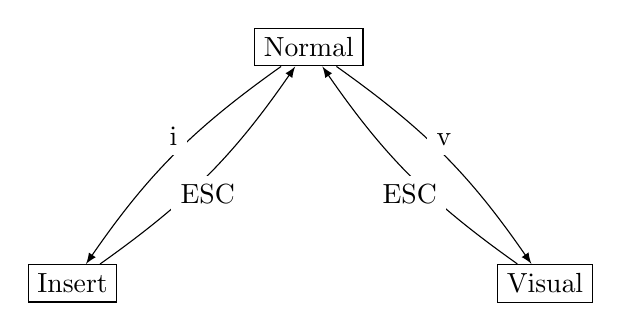
\begin{tikzpicture}
      \node[draw] at (0,-3) (insert) {Insert};
      \node[draw] at (3,0) (normal) {Normal};
      \node[draw] at (6,-3) (visual) {Visual};

      \draw[-latex] (normal) to[bend right=10] node[above,fill=white]{i} (insert);
      \draw[-latex] (normal) to[bend left=10] node[above,fill=white]{v} (visual);

      \draw[-latex] (insert) to[bend right=10] node[below,fill=white]{ESC} (normal);
      \draw[-latex] (visual) to[bend left=10] node[below,fill=white]{ESC} (normal);
    \end{tikzpicture}
  \end{figure}
\end{frame}

\sssframe{모드}{Visual}
  \begin{description}
    \item[v] visual 모드, 문자 하나씩 선택할 수 있음
    \item[C-v] v-block 모드, 블럭으로 선택할 수 있음
    \item[V] v-line 모드, 라인으로 선택할 수 있음
  \end{description}
\end{frame}

\ssframe{기본적인 움직임}
  \begin{description}
    \item[화살표] h($\leftarrow$) j($\downarrow$) k($\uparrow$) l($\rightarrow$)
    \item[문자] i(앞에 insert) a(뒤에 insert)
    \item[단어] b(\textbf{b}ack) w(\textbf{w}ord) e(\textbf{e}nd)
    \item[문장]
      \begin{itemize}
        \item I(문장 맨 앞에 insert) A(문장 맨 뒤에 insert)
        \item o(\textbf{o}pen, 문장 아래에 insert) O(문장 위에 insert)
        \item $\wedge$(문장 맨 앞으로) \$(문장 맨 뒤로) $\Rightarrow$ regex
      \end{itemize}
    \item[문단] \{(이전 문단) \}(다음 문단)
  \end{description}
\end{frame}

\ssframe{기본적인 커맨드 구조}
  (count +) action + (modifier +) range

  \begin{description}
    \item[count] 반복횟수
    \item[action]
      \begin{itemize}
          \item y: \textbf{y}ank
          \item d: \textbf{d}elete $\rightarrow$ 동시에 yank됨
          \item c: \textbf{c}hange
          \item v: \textbf{v}isual
      \end{itemize}
    \item[modifier]
      \begin{itemize}
          \item i: \textbf{i}nside
          \item a: \textbf{a}rround
      \end{itemize}
    \item[range] 움직임 + pair
  \end{description}
\end{frame}

\sssframe{기본적인 커맨드 구조}{예시1 - 움직임}
  \begin{itemize}
    \item \verb|vw|: 단어 하나 선택
      \begin{description}
        \item[v] visual
        \item[w] word \end{description}
    \item \verb|dw|: 단어 하나 삭제
      \begin{description}
        \item[d] delete
        \item[w] word
      \end{description}
    \item \verb|cw|: 단어 하나 변경
      \begin{description}
        \item[c] change
        \item[w] word
      \end{description}
  \end{itemize}
\end{frame}

\sssframe{기본적인 커맨드 구조}{예시2 - pair}
  \begin{itemize}
    \item \verb|vi}|: 중괄호 안쪽 선택
      \begin{description}
        \item[v] visual
        \item[i] inside
        \item[\}] 중괄호
      \end{description}
    \item \verb|va}|: 중괄호 포함 선택
      \begin{description}
        \item[v] visual
        \item[a] around
        \item[\}] 중괄호
      \end{description}
  \end{itemize}
\end{frame}

\ssframe{몇몇 유용한 커맨드}
  \begin{description}
    \item[dd] 문장 삭제
    \item[gg] 맨위로
    \item[G] 맨아래로
    \item[C-o] \textbf{o}ut, 이전 위치로
    \item[C-i] \textbf{i}n, 다음 위치로
    \item[zf] \textbf{f}old
    \item[zo] \textbf{o}pen
  \end{description}
\end{frame}

\ssframe{매크로}
  \begin{itemize}
    \item \verb|q<register><commands>q|
    \item \verb|@<register>|
  \end{itemize}
\end{frame}

\ssframe{설정파일}
  \verb|~/.config/nvim/init.vim|

  \begin{minted}{vim}
    let mapleader = ";"

    runtime vim/others.vim
  \end{minted}

  \verb|~/.config/nvim/vim/others.vim|

  \begin{minted}{vim}
    imap <silent>,d <ESC>

    set wildmenu
    set ignorecase
    set smartcase
    set hlsearch
    set incsearch

    set number

    set autoindent expandtab tabstop=2 shiftwidth=2
  \end{minted}
\end{frame}

\sssframe{설정파일}{lua}
  \verb|~/.config/nvim/init.vim|

  \begin{minted}{vim}
    ...

    lua require('boot')
  \end{minted}

  \verb|~/.config/nvim/lua/boot.lua|

  \begin{minted}{lua}
    vim.api.nvim_command('echo "lua loaded"')
  \end{minted}
\end{frame}

\ssframe{플러그인 매니저}
  \begin{description}
    \item[vim-plug] 
      \begin{itemize}
        \item 속도가 빠름
        \item \url{https://github.com/junegunn/vim-plug}
      \end{itemize}
    \item[\textbf{packer.nvim}] \url{https://github.com/wbthomason/packer.nvim}
  \end{description}
\end{frame}

\sssframe{플러그인 매니저}{설치}
  \verb|Shell|

  \begin{minted}[bgcolor=LightGray]{sh}
  git clone --depth 1\
    https://github.com/wbthomason/packer.nvim\
    ~/.local/share/nvim/site/pack/packer/start/packer.nvim
  \end{minted}

  \verb|~/.config/nvim/lua/boot.lua|

  \begin{minted}{lua}
  require('plugins')
  \end{minted}

  \verb|~/.config/nvim/lua/plugins.lua|

  \begin{minted}{lua}
  vim.cmd [[packadd packer.nvim]]

  return require('packer').startup(function(use)
    use 'wbthomason/packer.nvim'
  end)
  \end{minted}
\end{frame}

\sssframe{플러그인 매니저}{패키지 추가하기}
  \verb|~/.config/nvim/lua/plugins.lua|

  \begin{minted}{lua}
  return require('packer').startup(function(use)
    use 'wbthomason/packer.nvim'

    use 'username/reponame'
  end)
  \end{minted}

  \begin{description}
    \item[install] \verb|:PackerInstall|
    \item[sync] \verb|:PackerSync|
    \item[clean] \verb|:PackerClean|
  \end{description}
\end{frame}

\ssssframe{플러그인 매니저}{패키지 추가하기}{chadtree}
  \url{https://github.com/ms-jpq/chadtree}

  \verb|~/.config/nvim/lua/plugins.lua|

  \begin{minted}{lua}
    use {
      'ms-jpq/chadtree',
      branch = 'chad',
      run = 'python3 -m chadtree deps',
    }
  \end{minted}

  \verb|~/.config/nvim/vim/others.vim|

  \begin{minted}{vim}
    ...

    nmap <silent><leader>e :CHADopen<CR>
  \end{minted}
\end{frame}

\ssssframe{플러그인 매니저}{패키지 추가하기}{tree-sitter}
  \url{https://github.com/nvim-treesitter/nvim-treesitter}

  \verb|~/.config/nvim/lua/boot.lua|

  \begin{minted}{lua}
  ...

  require('others')
  \end{minted}

  \verb|~/.config/nvim/lua/others.lua|

  \begin{minted}{lua}
  require('nvim-treesitter.configs').setup {
    highlight = { enable = true },
  }
  \end{minted}
\end{frame}

\ssssframe{플러그인 매니저}{패키지 추가하기}{nvim-lspconfig}
  \url{https://github.com/neovim/nvim-lspconfig}
\end{frame}

\ssssframe{플러그인 매니저}{패키지 추가하기}{이외에 유용한 플러그인들}
  \begin{itemize}
    \item \url{https://github.com/nvim-telescope/telescope.nvim}
    \item \url{https://github.com/numToStr/Comment.nvim}
    \item \url{https://github.com/lukas-reineke/indent-blankline.nvim}
    \item \url{https://github.com/airblade/vim-gitgutter}
  \end{itemize}
\end{frame}

\begin{frame}
  EOF
\end{frame}

\end{document}
